\section{Methodology}

\subsection{Data Preparation}
To prepare the data for the active learning rare class discovery algorithm, we applied various dimensionality reduction techniques. Specifically, we generated the following data representations:
\begin{itemize}
    \item PCA with 2, 3, 4, and 5 components
    \item t-SNE with 2 and 3 components
    \item Raw data (no dimensionality reduction)
\end{itemize}

The resulting data representations and their corresponding labels were stored in the prepared data list, and the titles for these representations were stored in the data titles list.

\subsection{Active Learning Rare Class Discovery}
For the active learning rare class discovery algorithm, we implemented the following query strategies:
\begin{itemize}
    \item Uncertainty Sampling
    \item KNN Density-based Sampling (with k=3, k=10, and varying sigma)
    \item Oscillating KNN Density-based Sampling
    \item Random Sampling
\end{itemize}
These query strategies were stored in the \texttt{strategies} list.

Additionally, we used the following classifier models for the active learning algorithm:
\begin{itemize}
    \item K-Nearest Neighbors (with k=3 and k=10)
    \item Random Forest
    \item Support Vector Machine
\end{itemize}
These models were stored in the \texttt{models} list.

\subsection{Visualization}
To gain insights into the structure of the datasets, we visualized the data using 2D and 3D t-SNE projections. The 2D t-SNE plots are shown in Figure~\ref{fig:tsne_2d}, and the 3D t-SNE plots are shown in Figure~\ref{fig:tsne_3d}. The 3D t-SNE visualization is also provided as a MP4 movie to allow for interactive exploration of the data.

\begin{figure}[htbp]
\centering
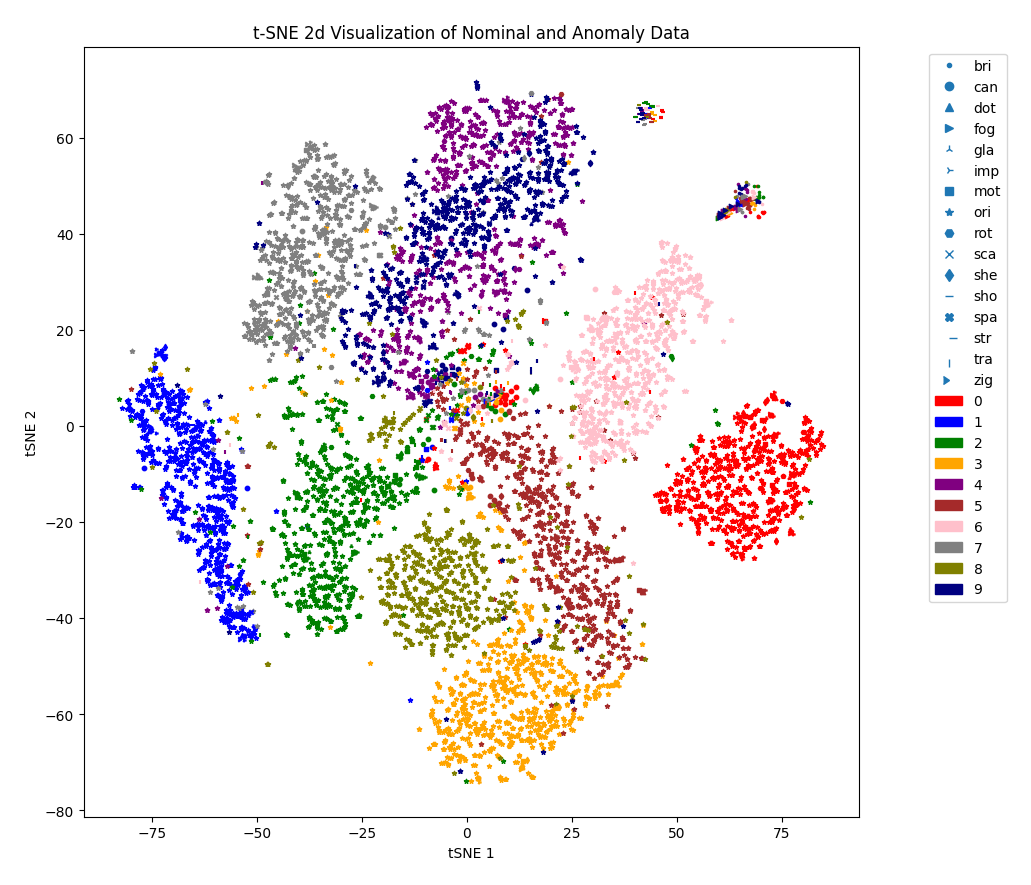
\includegraphics[width=0.5\textwidth]{resources/images/tsne_2d.png}
\caption{2D t-SNE Visualization of the Dataset}
\label{fig:tsne_2d}
\end{figure}

\begin{figure}[htbp]
\centering
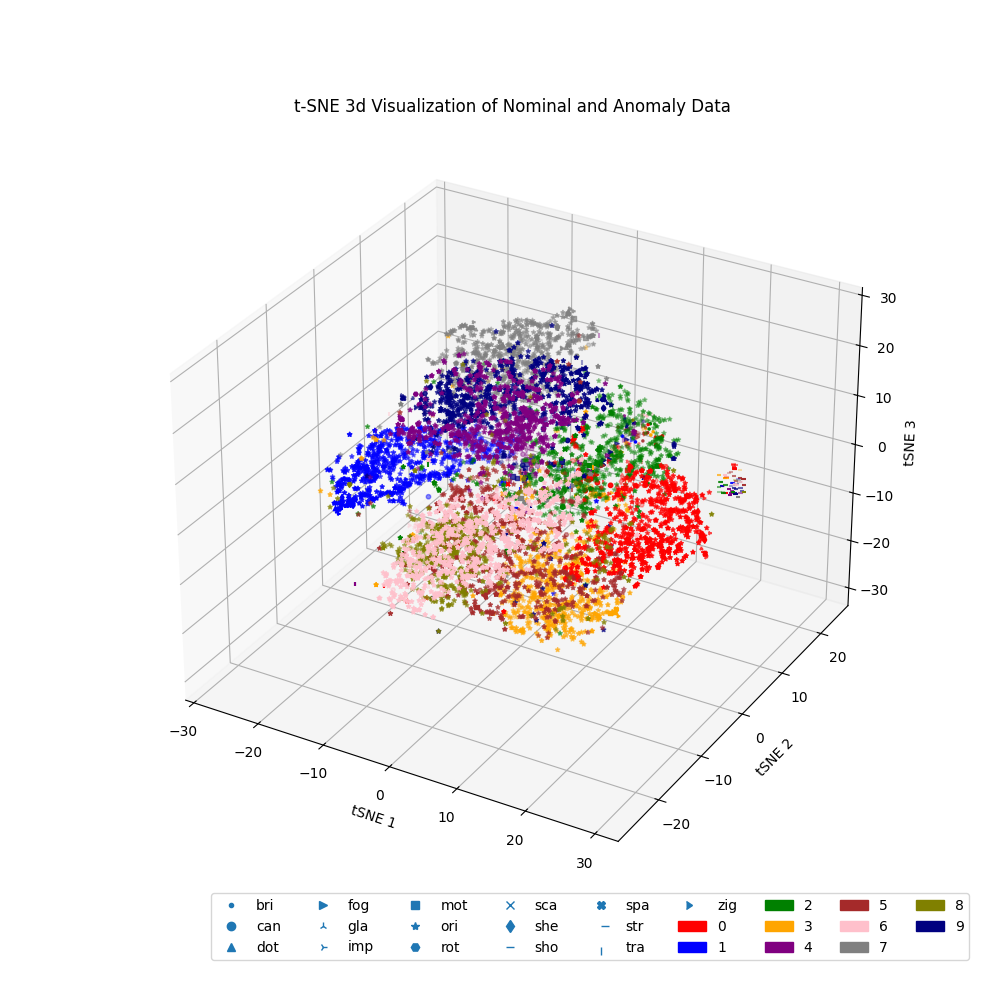
\includegraphics[width=0.5\textwidth]{resources/images/tsne_3d.png}
\caption{3D t-SNE Visualization of the Dataset}
\label{fig:tsne_3d}
\end{figure}